\documentclass{fkssolpub}

\usepackage[czech]{babel}
\usepackage{fontspec}
\usepackage{fkssugar}
\usepackage{amsmath}
\usepackage{graphicx}

\author{Ondřej Sedláček}
\school{Gymnázium Oty Pavla} 
\series{2p}
\problem{1} 

\begin{document}

Řešení je na obrázku níže. Jak je vidět, musel to být čtvereček v prvním
sloupci na čtvrtém řádku. Levý útvar je vůči druhému shodnému útvaru přetočen
o devadesát stupňů doprava.

\begin{figure}[h!]
	\centering
	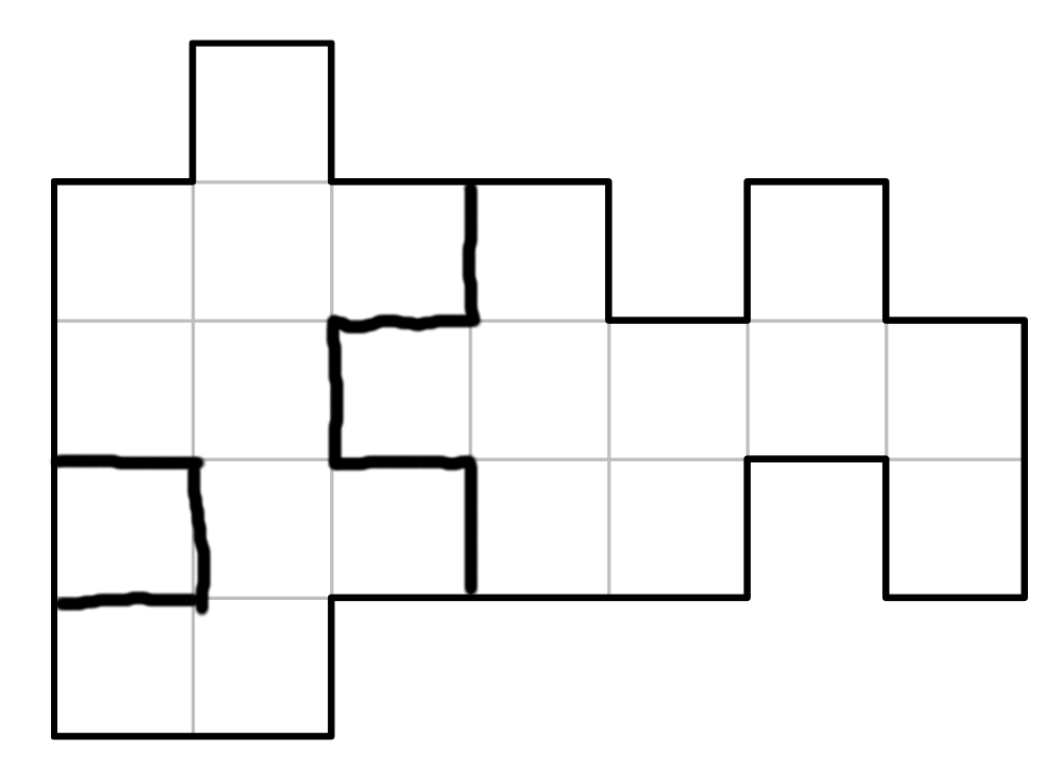
\includegraphics[width=\textwidth]{1.png}
	\caption{Řešení}
\end{figure}


\end{document}
